% Permission is granted to copy, distribute and/or modify this document
% under the terms of the GNU Free Documentation License, Version 1.3
% or any later version published by the Free Software Foundation;
% with no Invariant Sections, no Front-Cover Texts, and no Back-Cover Texts.
% A copy of the license is included in the section entitled "GNU
% Free Documentation License".
%
% Written (C) 2012 Michal Uricar

%% My macros %%
\def\##1{\relax\ifmmode\mathchoice      % italic bold vector, e.g. $\#{x}$
{\mbox{\boldmath$\displaystyle#1$}}
{\mbox{\boldmath$\textstyle#1$}}
{\mbox{\boldmath$\scriptstyle#1$}}
{\mbox{\boldmath$\scriptscriptstyle#1$}}\else
\hbox{\boldmath$\textstyle#1$}\fi}
%\def\##1{\mbox{\boldmath$\displaystyle#1$}}
\def\m#1{\mathbf{#1}}                  % bold matrix, e.g. $\m{A}$
\def\Re{{\mathbb R}}
\def\calS{{\cal S}}
\def\calO{{\cal O}}
\def\SY{{\cal Y}}
\def\SX{{\cal X}}
\def\Na{{\cal N}}
\def\calI{{\cal I}}
\def\calX{{\cal X}}
\def\col{{\rm col}}
\def\lz{\langle}
\def\pz{\rangle}
\def\equ#1{(\ref{#1})}
\def\ass{\mathrel {:=}}
\def\argmax{\mathop{\rm argmax}}
\def\argmin{\mathop{\rm argmin}}
\def\veps{\varepsilon}

\chapter{Bundle Methods for Regularized Risk Minimization}

In this chapter we describe learning algorithms related to convex regularized risk minimization, that are available in the \shogun{} toolbox. We begin with a brief outline of the convex regularized risk minimization problem in Section~\ref{sec:crrm}. Then, in Section~\ref{sec:bmrm}, we describe the bundle methods algorithms for solving this problem.

\section{Convex Regularized Risk Minimization} \label{sec:crrm}

Learning predictors from data is a standard machine learning task. A numerous such tasks are formulated as a convex quadratically regularized risk minimization problem.
%
\begin{equation}
	\#w^* = \arg\min_{\#w \in \mathbb{R}^n} F(\#w) := \left[ \frac{\lambda}{2} \| \#w  \|^2_2  + R(\#w) \right] \quad. \label{eq:learning_task}
\end{equation}
%
The objective function $F:\mathbb{R}^n \rightarrow \mathbb{R}$, often called regularized risk, is a sum of the quadratic regularization term and a convex empirical risk $R:\mathbb{R}^n \rightarrow \mathbb{R}$. The scalar $\lambda > 0$ is a pre-defined regularization constant and $\#w \in \mathbb{R}^n$ is a weight vector to be learned. The quadratic regularization term is added to improve the generalization. The empirical risk evaluates a match between the training examples and the weight vector $\#w$. It is often given as a sum of convex functions $r_i: \mathbb{R}^n \rightarrow \mathbb{R}$, i.e. the risk is given as follows
%
\begin{equation}
	R(\#w) = \sum_{i=1}^m r_i(\#w) \quad.
\end{equation}
%
We are interested especially in such instances of the learning task~\equ{eq:learning_task}, where the evaluation of the risk functions $r_i(\#w)$ is hard but still tractable.

In particular, one can use this technique for learning the Structured Output Support Vector Machine (SO-SVM) classifiers. The formulation of the learning task for SO-SVM (\cite{Tsoch-StructOutput05}) is as follows: given a training set of examples of input-output pairs $\{ (x_i, y_i) \}_1^m \in (\mathcal{X} \times \mathcal{Y})^m$, which are assumed to be i.i.d. from an unknown p.d.f. $p(x, y)$, we want to learn a weight vector $\#w \in \mathbb{R}^n$ of a linear classifier
%
\begin{equation}
	h(x; \#w) = \arg\max_{y \in \mathcal{Y}} \left\lz \#w, \Psi(x, y)  \right\pz \quad ,
\end{equation}
%
where $\Psi:\mathcal{X} \times \mathcal{Y} \rightarrow \mathbb{R}^n$ is a fixed mapping from the input-output space onto the parameters space. The goal is to find the weight vector $\#w$ which minimizes the expected risk $E_{p(x, y)}[\ell(y, h(x; \#w))]$ for a given non-negative loss function $\ell: \mathcal{Y} \times \mathcal{Y} \rightarrow \mathbb{R}_0^+$. Since the minimization of the expected risk is not possible due to unknown $p(x, y)$, we are minimizing \equ{eq:learning_task} which was shown to be a good approximation. The functions $r_i(\#w)$ are approximated using margin rescaling of the loss $\ell(y_i, h(x_i; \#w))$
%
\begin{equation}
	r_i(\#w) = \max_{y \in \mathcal{Y}} \left[ \ell(y_i, y) + \lz \#w, \Psi(x_i, y) - \Psi(x_i, y_i)  \pz  \right] \quad.
\end{equation}
%
%The Bundle Methods algorithms are modular and need only function that evaluates the value of the risk function $R(\#w)$ and the sub-gradient at given point $R'(\#w)$.
The sub-gradient at given point $R'(\#w)$ can be computed using the Danskin's theorem as $r_i(\#w) = \Psi(x_i, \hat{y}_i) - \Psi(x_i, y_i)$, where
\begin{equation}
	\hat{y}_i = \arg\max_{y \in \mathcal{Y}} \left[ \ell(y_i, y) + \lz \#w, \Psi(x_i, y)  \pz  \right]  \quad.
\end{equation}
%
Which corresponds to finding the most violated output for a given example.

Evaluation of $R(\#w)$ and $R'(\#w)$ is often expensive due to a possibly huge cardinality of the output set $\mathcal{Y}$, e.g. $\mathcal{Y}$ can be a set of all segmentations of an input image $x \in \mathcal{X}$. The SO-SVM learning problem~\equ{eq:learning_task} can be transformed to the equivalent quadratic program with the number of constraints linearly proportional to the number of classifier outputs $|\mathcal{Y}|$.

We can split approaches solving the SO-SVM learning problem into two main classes: {\sl approximate on-line algorithms} and {\sl precise methods}. The approximative methods are usually fast, especially at the early optimization stages, but they do not have a clear stopping condition. Moreover they require sophisticated setting of the learning rate and are also sensitive to improperly scaled data. Whereas the precise methods are slow, but they do have theoretically grounded stopping condition based on the optimality certificate. In the next section, we provide description of the recently most popular precise solver for the instances of SO-SVM learning problem~\equ{eq:learning_task}, i.e. the Bundle Methods for Regularized Risk Minimization (BMRM) proposed by \cite{Teo-BMRM-JMLR10}. The algorithm is implemented in \shogunclass{CDualLibQPBMSOSVM}.

\section{Bundle Methods for Regularized Risk Minimization} \label{sec:bmrm}

The main reason why the learning task \equ{eq:learning_task} is hard lies on the risk term $R(\#w)$, which is typically non-differentiable and its evaluation is expensive. The core idea of BMRM is replacing the complex $R(\#w)$ by its simpler cutting plane model $R_t(\#w)$
%
\begin{equation}
	R_t(\#w) = \max_{i=0,\dots, t-1} \left[ R(\#w_i) + \lz R'(\#w_i), \#w - \#w_i  \pz  \right] \quad,
\end{equation}
%
is defined as a point wise maximum over $t$ linear under-estimators, so called {\sl cutting planes}. $R'(\#w) \in \partial_{\#w_i} R(\#w_i)$ is an arbitrary sub-gradient of risk at given point $\#w_i$. The $i$-th cutting plane is a linear lower bound on the risk function $R(\#w)$ tight at the point $\#w_i$. The cutting plane approximation idea is illustrated in Figure~\ref{fig:cutting_planes}. With this approximation, one can simply replace the original hard problem~\equ{eq:learning_task} by a simpler {\sl reduced problem}
%
\begin{equation}
	\#w_t = \arg\min_{\#w \in \mathbb{R}^n} F_t(\#w) := \frac{\lambda}{2} \| \#w  \|^2 + R_t(\#w) \quad. \label{eq:reduced_problem}
\end{equation}
%
The reduced problem objective $F_t(\#w)$ is obtained from the original problem objective $F(\#w)$ by replacing the risk with its cutting plane approximation, while the regularization term remained unchanged.

\begin{figure}[ht]
	\centering
	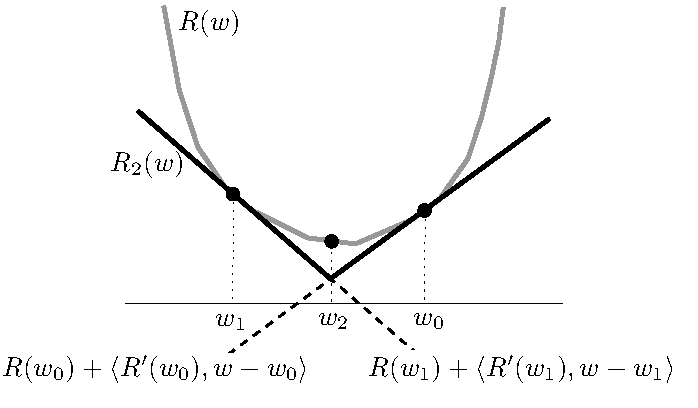
\includegraphics[width=0.7\linewidth]{fig/bmrm/cpmodel1}
	\caption{A convex function $R(\#w)$ can be approximated by a collection of linear under-estimators (cutting planes).}
	\label{fig:cutting_planes}
\end{figure}

Algorithm~\ref{alg:bmrm} outlines a pseudo-code of the standard BMRM.  It can be proved~\cite{Teo-BMRM-JMLR10}, that for arbitrary $\epsilon>0$, the BMRM returns a solution vector $\#w_t$ satisfying $F(\#w_t)  \leq F(\#w^*) + \epsilon$ after at most $\mathcal{O}(\frac{1}{\epsilon})$ iterations.

\begin{algorithm}[tb]
  \centering
  \caption{BMRM} \label{alg:bmrm}
  \begin{algorithmic}[1]
    \REQUIRE $\epsilon$, a function pointer $R(\#{w})$, a function pointer $R'(\#{w})$
    \STATE {\bf Initialization: } $\#{w} \leftarrow \mathbf{0}, t \leftarrow 0$
    \REPEAT
      %\STATE {\bf Initialization: } $\#{w} \leftarrow \mathbf{0}, t \leftarrow 0$
      \STATE $t \leftarrow t + 1$
      \STATE Compute $R(\#{w}_t), R'(\#{w}_t)$
      \STATE Update $R_t(\#{w}_t)$
      \STATE Solve $\#{w}_t \leftarrow \arg\min F_t(\#{w})$
      \STATE $\epsilon_t \leftarrow F(\#{w}_t) - F_t(\#{w}_t)$
    \UNTIL $\epsilon_t \le \epsilon$
  \end{algorithmic}
\end{algorithm}

In practice, the number of cutting planes $t$ required by the algorithm to converge is typically much lower than the dimensionality $n$ of the weight vector $\#w \in \mathbb{R}^n$. Therefore one can benefit from solving the reduced problem \equ{eq:reduced_problem} in its dual formulation. Let $\mathbf{A} = [\#a_0, \dots, \#a_{t-1}] \in \mathbb{R}^{n \times t}$ be matrix, whose columns are the sub-gradients $\#a_i = R'(\#w)$ and let $\#b = [b_0, \dots, b_{t-1}] \in \mathbb{R}^t$ be a column vector whose components are $b_i = R(\#w_i) - \lz R'(\#w_i), \#w_i \pz$. Then the Lagrange dual of~\equ{eq:reduced_problem} can be solved by the following quadratic program (QP):
%
\begin{equation}
	\#\beta_t \in \arg\max_{\#\beta \in \mathbb{R}^t} \left[ -\frac{1}{2\lambda} \#\beta^\top\mathbf{A}^\top\mathbf{A}\#\beta + \#\beta^\top\#b  \right],\quad \mathrm{s.t.}\quad \| \#\beta \|_1 = 1,\ \#\beta \ge 0
\end{equation}
%
And the primal solution can be obtained analytically by
%
\begin{equation}
	\#w_t = -\frac{1}{\lambda}\mathbf{A}\#\beta_t
\end{equation}
%
This algorithm is implemented in \shogunclass{libbmrm} and used by \shogunclass{CDualLibQPBMSOSVM} when the solver is set to be {\tt BMRM}.
